\documentclass{article}
\usepackage{graphicx}
\usepackage{amsmath}
\usepackage{geometry}
\geometry{a4paper, margin=1in}

\title{Wing Optimization Report}
\author{LLM Analysis}
\date{2025-06-12}

\begin{document}
\maketitle

\section*{Executive Summary}
This report summarizes the results and recommendations from an aerodynamic optimization performed on a wing design. The objective was to minimize drag at a cruise condition of $C_L = 0.5$, subject to geometric constraints of a wing area $S = 400 \text{ m}^2$ and span $b = 60 \text{ m}$. The design variables included taper, dihedral, twist, and sweep. The optimization was conducted using a Vortex Lattice Method (VLM) solver with the SLSQP algorithm.

\section{Optimization Results}

The optimization process successfully met the lift constraint of $C_L = 0.5$. The objective function, the drag coefficient ($C_D$), was minimized to 0.01093785. Key design variable values are as follows:

\begin{itemize}
    \item Taper ratio: The taper ratio reached its lower bound of 0.2, indicating the optimizer sought to minimize it as much as possible.
    \item Dihedral: The dihedral angle is 2.64 degrees.
    \item Twist: The twist distribution ranges from 1.64 to 2.41 degrees.
    \item Sweep: The sweep angle reached its upper bound of 30 degrees.
    \item Angle of Attack: The angle of attack settled at 3.94 degrees to achieve the desired $C_L$.
\end{itemize}

The lift distribution achieved is close to elliptical, which is in line with the objective of drag minimization. The optimization converged in 17 iterations with negligible wall clock time, suggesting acceptable performance of the SLSQP algorithm.

\section{Visualized Wing Optimization}
\begin{figure}[h!]
    \centering
    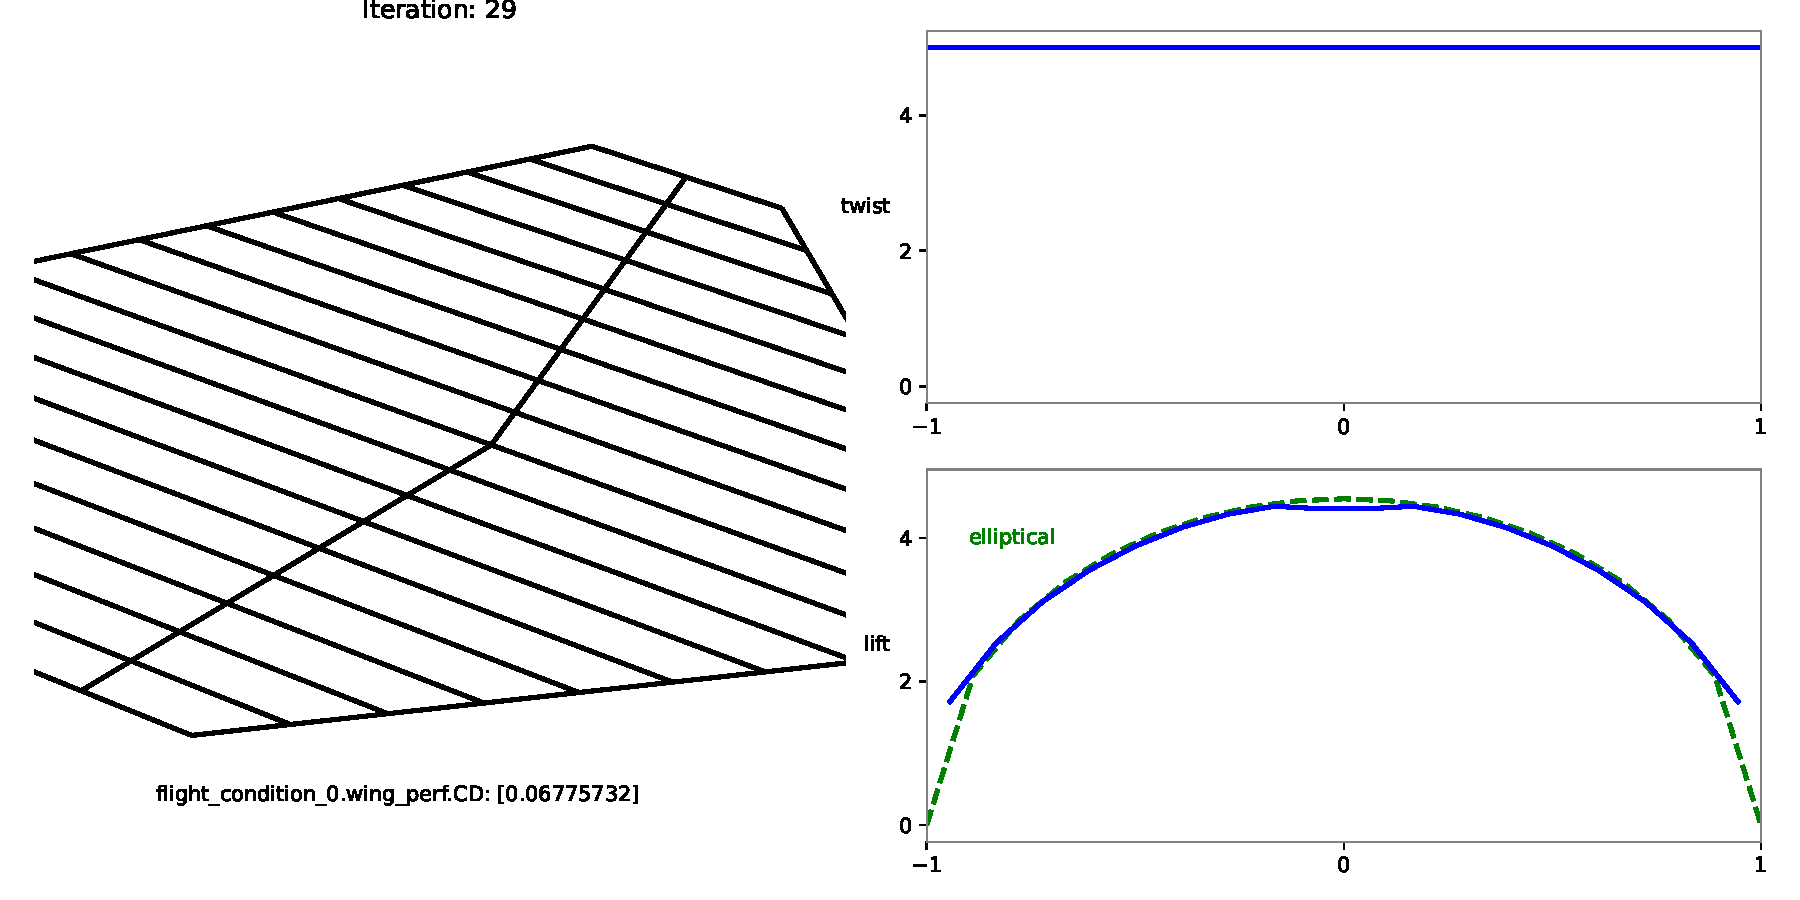
\includegraphics[width=0.7\textwidth]{./Optimized_Wing.pdf}
    \caption{Optimized Visualization of the Wing}
    \label{fig:optimized_wing}
\end{figure}

Figure \ref{fig:optimized_wing} shows the optimized wing design. Note the high sweep angle and the non-elliptical twist distribution. The lift distribution can be seen on the right side of the figure, where the elliptical lift distribution is shown for reference.

\section{Recommendations}
Based on the optimization results, the following recommendations are made:

\begin{enumerate}
    \item \textbf{Explore Lower Taper Ratios:} Since the taper ratio hit its lower bound, consider exploring even lower taper ratios. However, structural considerations must be taken into account to ensure the wing remains structurally sound. You may also want to consider moving the center of gravity forward.
    \item \textbf{Investigate Higher Sweep Angles:} Given that the sweep angle reached its upper bound, increasing this bound and re-running the optimization could potentially further reduce drag.
    \item \textbf{Refine Twist Distribution:} Further optimize the twist distribution to achieve a closer approximation of the ideal elliptical lift distribution. This may require a higher fidelity code such as a panel code or RANS simulation.
    \item \textbf{Consider a Multi-Point Optimization:} Optimizing for a single cruise condition might not be representative of the entire flight envelope. A multi-point optimization including other flight conditions (e.g., takeoff, landing, maneuver) would ensure more robust performance. Consider adding constraints to the lift coefficient at other flight conditions to help with the structural weight.
    \item \textbf{Add Structural Constraints:} Incorporate structural constraints, such as wing bending moment and shear force, to ensure the design is structurally feasible. Material and structural constraints should be included in the optimization process to potentially reduce the aircraft's mass. A structural solver, such as the one included in OpenAeroStruct, would be necessary.
    \item \textbf{Check Manufacturability:} Ensure the optimized geometry is manufacturable. Variables without constraints can lead to impractical designs, such as small tip chord areas that cannot accommodate ailerons. High twist can also pose manufacturing challenges. Therefore, include manufacturing constraints in future optimizations.
\end{enumerate}

\section{Limitations and Considerations}

\begin{itemize}
    \item The Vortex Lattice Method (VLM) is a low-fidelity aerodynamic solver and may not accurately capture complex flow phenomena such as stall, shock waves, and viscous effects. VLM is usually used for initial sizing and should be replaced with higher fidelity codes when available.
    \item The fixed wing area constraint may be problematic due to the number of design variables. It's often better to minimize the area, as less area typically results in less drag. In the future, the span and wing area should be active constraints using \texttt{prob.model.add\_constraint}.
    \item The aspect ratio, defined by the span and area constraints, significantly impacts stall characteristics and the shape of the lift distribution. Adjusting the aspect ratio can trade off performance and manufacturability.
    \item The final drag coefficient may be high due to the limitations of VLM, which primarily reduces induced drag and does not fully account for pressure drag. The high sweep angle may increase pressure drag.
\end{itemize}

\end{document}